
%% bare_conf.tex
%% V1.4b
%% 2015/08/26
%% by Michael Shell
%% See:
%% http://www.michaelshell.org/
%% for current contact information.
%%
%% This is a skeleton file demonstrating the use of IEEEtran.cls
%% (requires IEEEtran.cls version 1.8b or later) with an IEEE
%% conference paper.
%%
%% Support sites:
%% http://www.michaelshell.org/tex/ieeetran/
%% http://www.ctan.org/pkg/ieeetran
%% and
%% http://www.ieee.org/

%%*************************************************************************
%% Legal Notice:
%% This code is offered as-is without any warranty either expressed or
%% implied; without even the implied warranty of MERCHANTABILITY or
%% FITNESS FOR A PARTICULAR PURPOSE! 
%% User assumes all risk.
%% In no event shall the IEEE or any contributor to this code be liable for
%% any damages or losses, including, but not limited to, incidental,
%% consequential, or any other damages, resulting from the use or misuse
%% of any information contained here.
%%
%% All comments are the opinions of their respective authors and are not
%% necessarily endorsed by the IEEE.
%%
%% This work is distributed under the LaTeX Project Public License (LPPL)
%% ( http://www.latex-project.org/ ) version 1.3, and may be freely used,
%% distributed and modified. A copy of the LPPL, version 1.3, is included
%% in the base LaTeX documentation of all distributions of LaTeX released
%% 2003/12/01 or later.
%% Retain all contribution notices and credits.
%% ** Modified files should be clearly indicated as such, including  **
%% ** renaming them and changing author support contact information. **
%%*************************************************************************


% *** Authors should verify (and, if needed, correct) their LaTeX system  ***
% *** with the testflow diagnostic prior to trusting their LaTeX platform ***
% *** with production work. The IEEE's font choices and paper sizes can   ***
% *** trigger bugs that do not appear when using other class files.       ***                          ***
% The testflow support page is at:
% http://www.michaelshell.org/tex/testflow/



\documentclass[conference]{IEEEtran}
% Some Computer Society conferences also require the compsoc mode option,
% but others use the standard conference format.
%
% If IEEEtran.cls has not been installed into the LaTeX system files,
% manually specify the path to it like:
% \documentclass[conference]{../sty/IEEEtran}





% Some very useful LaTeX packages include:
% (uncomment the ones you want to load)


% *** MISC UTILITY PACKAGES ***
%
%\usepackage{ifpdf}
% Heiko Oberdiek's ifpdf.sty is very useful if you need conditional
% compilation based on whether the output is pdf or dvi.
% usage:
% \ifpdf
%   % pdf code
% \else
%   % dvi code
% \fi
% The latest version of ifpdf.sty can be obtained from:
% http://www.ctan.org/pkg/ifpdf
% Also, note that IEEEtran.cls V1.7 and later provides a builtin
% \ifCLASSINFOpdf conditional that works the same way.
% When switching from latex to pdflatex and vice-versa, the compiler may
% have to be run twice to clear warning/error messages.






% *** CITATION PACKAGES ***
%
%\usepackage{cite}
% cite.sty was written by Donald Arseneau
% V1.6 and later of IEEEtran pre-defines the format of the cite.sty package
% \cite{} output to follow that of the IEEE. Loading the cite package will
% result in citation numbers being automatically sorted and properly
% "compressed/ranged". e.g., [1], \cite{seznec2007tage}, \cite{calder1997evidence}, \cite{lee1995branch}, \cite{jimenez2001dynamic}, \cite{jimenez2003fast} without using
% cite.sty will become [1], \cite{calder1997evidence}, \cite{jimenez2001dynamic}--\cite{lee1995branch}, \cite{seznec2007tage} using cite.sty. cite.sty's
% \cite will automatically add leading space, if needed. Use cite.sty's
% noadjust option (cite.sty V3.8 and later) if you want to turn this off
% such as if a citation ever needs to be enclosed in parenthesis.
% cite.sty is already installed on most LaTeX systems. Be sure and use
% version 5.0 (2009-03-20) and later if using hyperref.sty.
% The latest version can be obtained at:
% http://www.ctan.org/pkg/cite
% The documentation is contained in the cite.sty file itself.






% *** GRAPHICS RELATED PACKAGES ***
%
\ifCLASSINFOpdf
  % \usepackage[pdftex]{graphicx}
  % declare the path(s) where your graphic files are
  % \graphicspath{{../pdf/}{../jpeg/}}
  % and their extensions so you won't have to specify these with
  % every instance of \includegraphics
  % \DeclareGraphicsExtensions{.pdf,.jpeg,.png}
\else
  % or other class option (dvipsone, dvipdf, if not using dvips). graphicx
  % will default to the driver specified in the system graphics.cfg if no
  % driver is specified.
  % \usepackage[dvips]{graphicx}
  % declare the path(s) where your graphic files are
  % \graphicspath{{../eps/}}
  % and their extensions so you won't have to specify these with
  % every instance of \includegraphics
  % \DeclareGraphicsExtensions{.eps}
\fi
% graphicx was written by David Carlisle and Sebastian Rahtz. It is
% required if you want graphics, photos, etc. graphicx.sty is already
% installed on most LaTeX systems. The latest version and documentation
% can be obtained at: 
% http://www.ctan.org/pkg/graphicx
% Another good source of documentation is "Using Imported Graphics in
% LaTeX2e" by Keith Reckdahl which can be found at:
% http://www.ctan.org/pkg/epslatex
%
% latex, and pdflatex in dvi mode, support graphics in encapsulated
% postscript (.eps) format. pdflatex in pdf mode supports graphics
% in .pdf, .jpeg, .png and .mps (metapost) formats. Users should ensure
% that all non-photo figures use a vector format (.eps, .pdf, .mps) and
% not a bitmapped formats (.jpeg, .png). The IEEE frowns on bitmapped formats
% which can result in "jaggedy"/blurry rendering of lines and letters as
% well as large increases in file sizes.
%
% You can find documentation about the pdfTeX application at:
% http://www.tug.org/applications/pdftex





% *** MATH PACKAGES ***
%
%\usepackage{amsmath}
% A popular package from the American Mathematical Society that provides
% many useful and powerful commands for dealing with mathematics.
%
% Note that the amsmath package sets \interdisplaylinepenalty to 10000
% thus preventing page breaks from occurring within multiline equations. Use:
%\interdisplaylinepenalty=2500
% after loading amsmath to restore such page breaks as IEEEtran.cls normally
% does. amsmath.sty is already installed on most LaTeX systems. The latest
% version and documentation can be obtained at:
% http://www.ctan.org/pkg/amsmath





% *** SPECIALIZED LIST PACKAGES ***
%
%\usepackage{algorithmic}
% algorithmic.sty was written by Peter Williams and Rogerio Brito.
% This package provides an algorithmic environment fo describing algorithms.
% You can use the algorithmic environment in-text or within a figure
% environment to provide for a floating algorithm. Do NOT use the algorithm
% floating environment provided by algorithm.sty (by the same authors) or
% algorithm2e.sty (by Christophe Fiorio) as the IEEE does not use dedicated
% algorithm float types and packages that provide these will not provide
% correct IEEE style captions. The latest version and documentation of
% algorithmic.sty can be obtained at:
% http://www.ctan.org/pkg/algorithms
% Also of interest may be the (relatively newer and more customizable)
% algorithmicx.sty package by Szasz Janos:
% http://www.ctan.org/pkg/algorithmicx




% *** ALIGNMENT PACKAGES ***
%
%\usepackage{array}
% Frank Mittelbach's and David Carlisle's array.sty patches and improves
% the standard LaTeX2e array and tabular environments to provide better
% appearance and additional user controls. As the default LaTeX2e table
% generation code is lacking to the point of almost being broken with
% respect to the quality of the end results, all users are strongly
% advised to use an enhanced (at the very least that provided by array.sty)
% set of table tools. array.sty is already installed on most systems. The
% latest version and documentation can be obtained at:
% http://www.ctan.org/pkg/array


% IEEEtran contains the IEEEeqnarray family of commands that can be used to
% generate multiline equations as well as matrices, tables, etc., of high
% quality.




% *** SUBFIGURE PACKAGES ***
%\ifCLASSOPTIONcompsoc
%  \usepackage[caption=false,font=normalsize,labelfont=sf,textfont=sf]{subfig}
%\else
%  \usepackage[caption=false,font=footnotesize]{subfig}
%\fi
% subfig.sty, written by Steven Douglas Cochran, is the modern replacement
% for subfigure.sty, the latter of which is no longer maintained and is
% incompatible with some LaTeX packages including fixltx2e. However,
% subfig.sty requires and automatically loads Axel Sommerfeldt's caption.sty
% which will override IEEEtran.cls' handling of captions and this will result
% in non-IEEE style figure/table captions. To prevent this problem, be sure
% and invoke subfig.sty's "caption=false" package option (available since
% subfig.sty version 1.3, 2005/06/28) as this is will preserve IEEEtran.cls
% handling of captions.
% Note that the Computer Society format requires a larger sans serif font
% than the serif footnote size font used in traditional IEEE formatting
% and thus the need to invoke different subfig.sty package options depending
% on whether compsoc mode has been enabled.
%
% The latest version and documentation of subfig.sty can be obtained at:
% http://www.ctan.org/pkg/subfig




% *** FLOAT PACKAGES ***
%
%\usepackage{fixltx2e}
% fixltx2e, the successor to the earlier fix2col.sty, was written by
% Frank Mittelbach and David Carlisle. This package corrects a few problems
% in the LaTeX2e kernel, the most notable of which is that in current
% LaTeX2e releases, the ordering of single and double column floats is not
% guaranteed to be preserved. Thus, an unpatched LaTeX2e can allow a
% single column figure to be placed prior to an earlier double column
% figure.
% Be aware that LaTeX2e kernels dated 2015 and later have fixltx2e.sty's
% corrections already built into the system in which case a warning will
% be issued if an attempt is made to load fixltx2e.sty as it is no longer
% needed.
% The latest version and documentation can be found at:
% http://www.ctan.org/pkg/fixltx2e


%\usepackage{stfloats}
% stfloats.sty was written by Sigitas Tolusis. This package gives LaTeX2e
% the ability to do double column floats at the bottom of the page as well
% as the top. (e.g., "\begin{figure*}[!b]" is not normally possible in
% LaTeX2e). It also provides a command:
%\fnbelowfloat
% to enable the placement of footnotes below bottom floats (the standard
% LaTeX2e kernel puts them above bottom floats). This is an invasive package
% which rewrites many portions of the LaTeX2e float routines. It may not work
% with other packages that modify the LaTeX2e float routines. The latest
% version and documentation can be obtained at:
% http://www.ctan.org/pkg/stfloats
% Do not use the stfloats baselinefloat ability as the IEEE does not allow
% \baselineskip to stretch. Authors submitting work to the IEEE should note
% that the IEEE rarely uses double column equations and that authors should try
% to avoid such use. Do not be tempted to use the cuted.sty or midfloat.sty
% packages (also by Sigitas Tolusis) as the IEEE does not format its papers in
% such ways.
% Do not attempt to use stfloats with fixltx2e as they are incompatible.
% Instead, use Morten Hogholm'a dblfloatfix which combines the features
% of both fixltx2e and stfloats:
%
% \usepackage{dblfloatfix}
% The latest version can be found at:
% http://www.ctan.org/pkg/dblfloatfix




% *** PDF, URL AND HYPERLINK PACKAGES ***
%
%\usepackage{url}
% url.sty was written by Donald Arseneau. It provides better support for
% handling and breaking URLs. url.sty is already installed on most LaTeX
% systems. The latest version and documentation can be obtained at:
% http://www.ctan.org/pkg/url
% Basically, \url{my_url_here}.
\usepackage{algorithm}
\usepackage{algpseudocode}
\usepackage{amsmath}
\usepackage{amsmath,amssymb,amsthm,latexsym,paralist, booktabs}
\usepackage{url}
\usepackage[pdftex]{graphicx}
\usepackage{subfigure}
% default pic path
\graphicspath{{pics/}}




% *** Do not adjust lengths that control margins, column widths, etc. ***
% *** Do not use packages that alter fonts (such as pslatex).         ***
% There should be no need to do such things with IEEEtran.cls V1.6 and later.
% (Unless specifically asked to do so by the journal or conference you plan
% to submit to, of course. )


% correct bad hyphenation here
\hyphenation{op-tical net-works semi-conduc-tor}


\begin{document}
%
% paper title
% Titles are generally capitalized except for words such as a, an, and, as,
% at, but, by, for, in, nor, of, on, or, the, to and up, which are usually
% not capitalized unless they are the first or last word of the title.
% Linebreaks \\ can be used within to get better formatting as desired.
% Do not put math or special symbols in the title.
\title{Yet Another Implementation of Re-Reference Interval Prediction (RRIP) Cache Replacement}


% author names and affiliations
% use a multiple column layout for up to three different
% affiliations
\author{\IEEEauthorblockN{Yukun Zeng}
\IEEEauthorblockA{Department of Computer Science and Engineering\\
Texas A\&M University\\
College Station, TX 77840\\
Email: yzeng@tamu.edu}}

% conference papers do not typically use \thanks and this command
% is locked out in conference mode. If really needed, such as for
% the acknowledgment of grants, issue a \IEEEoverridecommandlockouts
% after \documentclass

% for over three affiliations, or if they all won't fit within the width
% of the page, use this alternative format:
% 
%\author{\IEEEauthorblockN{Michael Shell\IEEEauthorrefmark{1},
%Homer Simpson\IEEEauthorrefmark{2},
%James Kirk\IEEEauthorrefmark{3}, 
%Montgomery Scott\IEEEauthorrefmark{3} and
%Eldon Tyrell\IEEEauthorrefmark{4}}
%\IEEEauthorblockA{\IEEEauthorrefmark{1}School of Electrical and Computer Engineering\\
%Georgia Institute of Technology,
%Atlanta, Georgia 30332--0250\\ Email: see http://www.michaelshell.org/contact.html}
%\IEEEauthorblockA{\IEEEauthorrefmark{2}Twentieth Century Fox, Springfield, USA\\
%Email: homer@thesimpsons.com}
%\IEEEauthorblockA{\IEEEauthorrefmark{3}Starfleet Academy, San Francisco, California 96678-2391\\
%Telephone: (800) 555--1212, Fax: (888) 555--1212}
%\IEEEauthorblockA{\IEEEauthorrefmark{4}Tyrell Inc., 123 Replicant Street, Los Angeles, California 90210--4321}}




% use for special paper notices
%\IEEEspecialpapernotice{(Invited Paper)}




% make the title area
\maketitle

% As a general rule, do not put math, special symbols or citations
% in the abstract
\begin{abstract}
Cache replacement policies server on the purpose of predicting memory access patterns to make most of size limited cache space to reduce lags caused by too many memory accesses. Most early cache replacement policies like LRU simply predict the hit and miss blocks will be re-referenced immediately afterwards. Certainly applications  with distant re-reference interval, either due to a large working set or frequent bursts of references to non-temporal data (namely, scans), performs very badly on such policies. To properly adapt to these applications, researchers from Intel proposed a Re-Reference Interval Prediction (RRIP) based cache replacement policy, which can learn cache block re-reference patterns on-the-fly thereby providing scan and thrash resistancy.  The RRIP is shown in experiments to perform significantly better comparing to LRU, and the hardware budget it requires is practical (2X less than LRU, 2.5X less than LFU). In this paper, we present the design and our implementation of one NRU and two RRIP cache replacement policies. We also show a series of experiments carried out on the provided infrasctructure in comparison to other policies like LRU and NRU.
\end{abstract}

% no keywords




% For peer review papers, you can put extra information on the cover
% page as needed:
% \ifCLASSOPTIONpeerreview
% \begin{center} \bfseries EDICS Category: 3-BBND \end{center}
% \fi
%
% For peerreview papers, this IEEEtran command inserts a page break and
% creates the second title. It will be ignored for other modes.
\IEEEpeerreviewmaketitle



\section{Introduction}
\subsection{Cache and Replacement Policies}
Cache is an indispensable intermediate level storage in the memory hierarchy of modern computer architecture. It fills the great speed gap between high-performance processors and the main memory. Cache size is always limited due to the fact that it's too expensive, thus it can only take a small, frequently-used portion from main memory to feed the processor in a much quicker manner. Therefore, there must be some times that the processor want to access the portion of memory that is not currently available in cache (or a certain cache set it maps to), namely, this is a cache miss. Capacity miss is the case that at the meantime, the cache (or cache set) is full, which means we have to drop one block in the cache so that the new block can come in. Among all the miss circumstances, capacity miss is the biggest bottleneck that influences cache performance. Upon a capacity miss, we ideally want new blocks of memory to get into the cache by replacing old blocks that won't be accessed in the distant future. To achieve that, we need a cache replacement policy that makes choices on which block to abandon for new blocks.
\subsection{Motivation}
Practical replacement policies are not aware of the future re-reference sequence of memory blocks, thus they usually do replacement decisions based on prediction of which memory block (currently in cache) will be accessed again in the furthest future so that they could evict it for new block with minimum price. Specifically, the most widely-used replacement policy, namely Least Recently Used (LRU), maintains a chain (basically a timeline of memory blocks reference operations) and assumes the block that is accessed the earliest in the chain will be most unlikely to be re-reference again in the near-immediate. Apparently, such a policy performs good in applications with high data locality, but it cannot extend well to thrashing applications or applications with large working sets described before. Some other policies based on LRU have been proposed recently to achieve better miss rate or deal with different applications in \cite{jaleel2008adaptive} \cite{qureshi2007adaptive} \cite{srinath2007feedback} \cite{xie2009pipp}. 

In last-level cache (LLC), the accuracy of a replacement policy is crucial since a miss in the last-level means an access to main memory. As we mentioned before, pure LRU policy has several disadvantages and many studies like \cite{kaxiras2001cache} \cite{lai2001dead} \cite{qureshi2007adaptive} \cite{xie2009pipp} have illustrated that temporal locality filtering by small front-level caches cause lots of blocks that will never be re-referenced again evicted to LLC. We now study the worst cases of LRU in the following memory access patterns:
\begin{itemize}
	\item Recency-friendly Access Patterns
	\item Thrashing Access Patterns
	\item Streaming Access Patterns
	\item Mixed Access Patterns
\end{itemize} 
\cite{jaleel2010high} has illustrated that for both thrashing and mixed access patterns, there is room to improve LRU. The key to this improvement shall rely on a better prediction on re-reference interval of different memory blocks based on historical reference information.

Though designed to describe the recency of block references, we can also regard LRU timeline as a RRIP chain in the sense that the LRU policy is actually assuming the head block of its chain will be re-referenced near-immediate while the tail will have a distant re-reference interval. According the relations between RRIP and LRU above, we can adapt LRU to more kinds of applications by applying RRIP policy into it to learn and predict the re-reference patterns of blocks on-the-fly.

\section{Related Works}
In computer architecture literature, cache replacement policies have been studied intensively. For the fact that our policy aims at improving LLC performance, we present a brief review on prior art on this topic. Problems of dead blocks (blocks that are never or distantly accessed after brought into cache) is commonly solved by introducing block access frequency to predict re-reference pattern. Recency and frequency are two factors mostly used to determine the re-reference pattern of a block. Leveraging counters to record access frequencies of blocks,  Least Frequently Used (LFU) \cite{lee2001lrfu} predicts that the block being accessed most frequently will be referenced earliest in the future. However, LFU only considers the frequency factors, it's easy to imagine that when some applications have finished and new applications come along, it will lead to continuous cache misses for a considerably long time due to the unawareness of recency. To address the problems with high recency applications, studies in \cite{lee2001lrfu} \cite{o1993lru} \cite{robinson1990data} combined both factors of recency and frequency but they require parameter tuning beforehand when dealing with different workloads. Self-tuning policies proposed in \cite{megiddo2003arc} \cite{bansal2004car} \cite{subramanian2006adaptive}, though effective and adaptive to various workloads, they significantly increased the hardware complexity and overhead. On the other hand, \cite{liu2008cache} proposed to combine dead blocks predictions with replacement policies at LLC. As \cite{qureshi2007adaptive} showed that the occurence of dead blocks often happens in the case when working set is larger that cache size, Dynamic Insertion Policy (DIP) is also proposed to dynamically change insertion policy while the workloads vary. Different from using a common recency stack, pseudo-LIFO \cite{chaudhuri2009pseudo} uses fill stack to learn the re-reference probabilities of a block but it requires additional hardware to track fill stack positions. Similarly to pseudo-LIFO, other solutions in \cite{basu2007scavenger} \cite{johnson1994x3} \cite{loh2009extending} \cite{rajan2007emulating} \cite{zhou2001multi} requires significant changes or additions on current cache hardware implementation.


\section{Methodology}
As discussed before, in the cases of mixed access pattern and thrashing accesses, LRU's performance is greatly undermined. To improve the replacement policy in such circumstances, [RRIP] mainly proposed two Static RRIP (SRRIP) policies, one uses hit promotion strategy which predicts every hit block will be accessed in the near-immediate, the other maintains a multi-bit counter to exploit block access frequency. The original paper also has proposed a Bimodal RRIP (BRRIP) that is suitable for predicting with thrash-resistancy, it was also combined with SRRIP using Set Dueling \cite{qureshi2007adaptive} so that we can dynamically determine the type of current workloads and switch between two policies to achieve a better overall performance. However, this paper didn't go into details on BRRIP and DRRIP, thus we omit their implementation here and present the hit promotion and frequency priority strategy here, as well as the NRU policy, which serves as the similar role of benchmark as LRU.
\subsection{Not Recently Used (NRU) Replacement}
NRU replacement policy is an approximation of LRU which yields similar performance while is much simpler and requires less on hardware. Different from LRU, who maintains a chain (which is actually a linked-list) and keeps doing complex operations like insertion and switching, NRU only requires single bit for predicting the future re-reference of cache blocks. A block with nru-bit of  `0' means it will be accessed in near-immediate, while nru-bit of `1' implies the block will be re-referenced after a distant interval. The detailed initialization, update and victim selection algorithm of NRU is provided in Algo \ref{nru_algo}.
\begin{algorithm}[!htp]
  \caption{\textsc{NRU Replacement Policy}}
  \label{nru_algo}
  \begin{algorithmic}
  \Function{Initialize}{}
	\State $setCount$ = number of sets in the cache
	\State $assoc$ = cache associativity
	\State init $replInfo[setCount][assoc]$
	\For{$setIndex = 0 \rightarrow (setCount - 1)$}
		\For{$blockIndex = 0 \rightarrow assoc$}
			\State $replInfo[setIndex][blockIndex].nru\_bit = 1$
		\EndFor
	\EndFor
  \EndFunction
  \Function{VictimSelection}{setIndex}
	\State $lineReplInfo = replInfo[setIndex]$
	\For{$blockIndex = 0 \rightarrow assoc$}
		\If{$lineReplInfo[blockIndex].nru\_bit == 1$}
			\State $lineReplInfo[blockIndex].nru\_bit = 0$
			\State \Return $blockIndex$
		\EndIf
	\EndFor
	\For{$blockIndex = 1 \rightarrow assoc$}
		\State $lineReplInfo[blockIndex].nru\_bit = 1$
	\EndFor
	\State \Return 0
  \EndFunction
  \Function{HitUpdate}{setIndex, blockIndex, cacheHit}
	\If{$cacheHit$}
		\State $replInfo[setIndex][blockIndex] = 0$
	\EndIf
	\State \Return 0
  \EndFunction
  \end{algorithmic}
\end{algorithm}
\subsection{Static RRIP (SRRIP)}
While we enjoy the simplicity of NRU replacement policy based on single bit hardware, the discreteness of NRU (predicts either near-immediate or distant re-reference) greatly limits its performance for mixed access patterns because scan blocks will always be predicted that they will be re-referenced near-immediate while in fact it's not ture. To correctly identify such scans and improve scan-resistancy, the authors proposed RRIP cache replacement policy that leverages $M$ bits to store $2^M$ Re-reference Prediction Values (RRPV). With decreasing RRPV values, the possibility of a block to be re-referenced in near-immediate gets bigger. Since prediction of either near-immediate or distant re-reference on a block is not robust shown in the NRU, RRIP inserts new blocks with a prediction that it would be accessed in a long re-reference interval. A long re-reference interval is defined to be $2^M - 2$. The idea is through a long re-reference setting we can prevent distant re-reference block from getting into the cache and it also buys the policy more time to learn re-reference intervals for different blocks.

Upon a cache replacement, the victim selection algorithm of RRIP policy iterate all the blocks in order to find the first block with a distant re-reference interval, i.e., whose RRPV equals distant re-reference interval ($2^M - 1$). If such block exists, then we simply replace it and set its RRPV to long re-reference value ($2^M - 2$). If the RRPV of all blocks is below distant re-reference interval, we iteratively increase the RRPV of all blocks and search again after each increment operation. 

The authors further proposed two different policies for updating RRPVs when cache hits, one named Hit Promotion while the other is based on Frequency Priority. In the following sections we briefly go through mechanisms in these two policies.
\subsubsection{RRIP-Hit Promotion}
RRIP hit promotion policy, abbreviated as RRIP-HP, prioritizes to replace blocks that are not receiving hits over any block that is re-referenced. When a cache hit happens, it predicts the block associated with the hit will be re-referenced in the near-immediate by setting RRPV of that block to be 0. The algorithms for RRIP-HP are given in Algo \ref{rrip_hp_algo}. Though RRIP-HP performs well in most workloads by predicting re-reference interval, it can potentially degrade performance in the case that a cache block is only referenced once after insertion (like what happens in a scan or thrash) since it will direcly set RRPV to be 0 which would make it a long time for this distant re-referenced block to be evicted.
\begin{algorithm}[!htp]
  \caption{\textsc{RRIP-HP Replacement Policy}}
  \label{rrip_hp_algo}
  \begin{algorithmic}
  \Function{Initialize}{M}
	\State $max\_rrpv = pow(2, M) - 1$
	\State $setCount$ = number of sets in the cache
	\State $assoc$ = cache associativity
	\State init $replInfo[setCount][assoc]$
	\For{$sIndex = 0 \rightarrow (setCount - 1)$}
		\For{$bIndex = 0 \rightarrow assoc$}
			\State $replInfo[sIndex][bIndex].rrpv = max\_rrpv$
		\EndFor
	\EndFor
  \EndFunction
  \Function{VictimSelection}{sIndex}
	\State $lineReplInfo = replInfo[sIndex]$
	\State $maxRrpvIndex = assoc$
	\For{$blockIndex = 0 \rightarrow assoc$}
		\If{$lineReplInfo[bIndex].rrpv = max\_rrpv$}
			\State $lineReplInfo[bIndex].rrpv = max\_rrpv - 1$
			\State \Return $bIndex$
		\EndIf
		\State $curRrpv = lineReplInfo[bIndex].rrpv$
		\State $maxRrpv = lineReplInfo[maxRrpvIndex].rrpv$
		\If{$curRrpv > maxRrpv$}
			\State $maxRrpvIndex = bIndex$
		\EndIf
	\EndFor
	\State $diff = max\_rrpv - lineReplInfo[maxRrpvIndex]$
	\For{$bIndex = 0 \rightarrow assoc$}
		\State $lineReplInfo[bIndex].rrpv += diff$
	\EndFor
	\State $lineReplInfo[maxRrpvIndex] = max\_rrpv - 2$
	\State \Return maxRrpvIndex
  \EndFunction
  \Function{HitUpdate}{sIndex, bIndex, cacheHit}
	\If{$cacheHit$}
		\State $replInfo[sIndex][bIndex] = 0$
	\EndIf
	\State \Return 0
  \EndFunction
  \end{algorithmic}
\end{algorithm}

\subsubsection{RRIP-Frequency Priority}
To properly address the disadvantages of RRIP-HP, we further implemented the RRIP frequency priority (RRIP-FP) policy. Since there are only some trivial changes between RRIP-HP and RRIP-FP, we omitted the detailed algorithm part of RRIP-FP. The biggest difference between RRIP-FP and RRIP-HP lies in that RRIP-FP decrements the RRPV values of hit blocks instead of setting them directly to zero (near-immediate). Apparently by applying such update policy, we will learn more information on the re-reference frequency of blocks thereby improving the performance based on RRIP-HP. 
\begin{figure*}
\begin{minipage}[!htbp]{1\linewidth}
\begin{center}
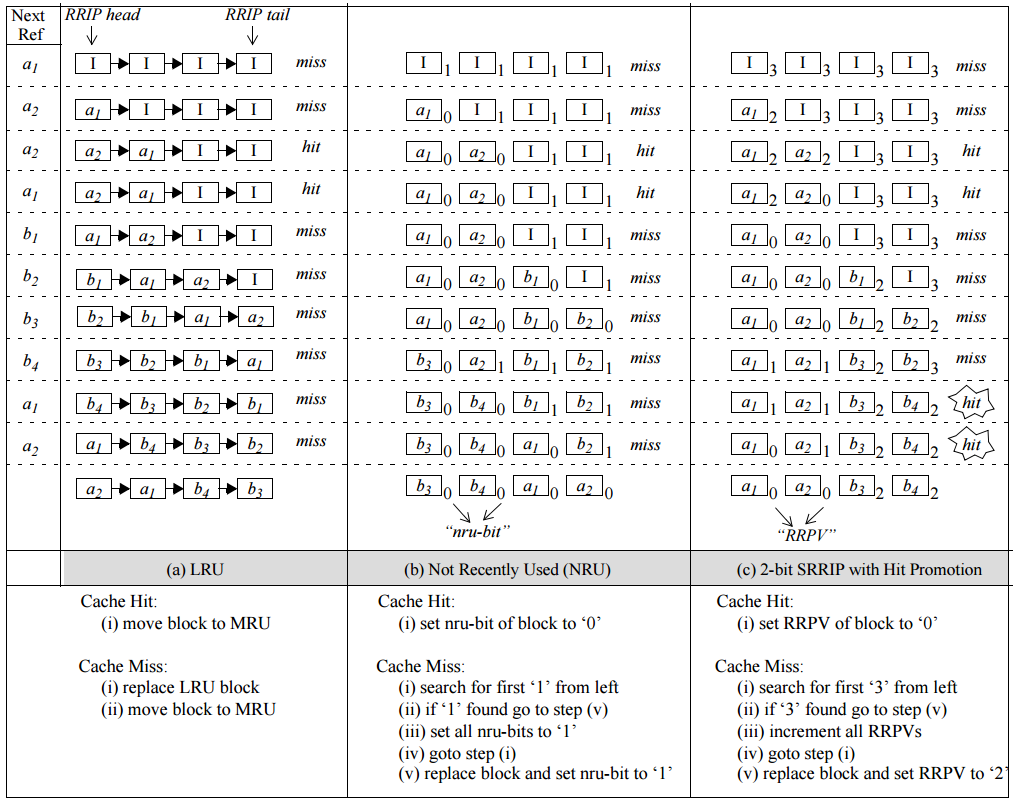
\includegraphics[width=1\textwidth]{policy_behavior.png} 
\caption{Behavior comparisons between LRU, NRU and SRRIP}\label{policy_behavior}
\end{center}	   
\end{minipage}
\end{figure*}

Since all the RRIP policies presented are static in the sense that they are not adaptive to different workloads, we refer them as Static Re-Reference Interval Prediction (SRRIP). A simple example provided in \cite{jaleel2010high} that illustrates the behavior of RRIP in comparison with LRU and NRU policy is also given in Figure \ref{policy_behavior}.



\section{Experiments}
In the experiment part, we carried out a comprehensive analysis on the performance of both HP and FP RRIP policies and normalized their results based on LRU performance, we also added NRU into consideration. First, we tune the $M$ parameter by running a series workloads on varying $M$ values, recall that $M$ is the number of bits we use for each cache block to store their re-reference frequency. Then we use the best fitted $M$ value and run benchmarks to get normalized performance improvements based on LRU (in some cases the improvement might be negative which means LRU outperforms new strategies). The metrics we used for evaluation includes both MPKI and IPC.
\subsection{RRIP Tuning}
We first tune the RRIP replacement policy by setting $M$ from 2 to 4 and comparing the results to NRU. Both the MPKI and IPC performance results of RRIP-HP and RRIP-FP are show in Figure \ref{rrip_perf}. From the figure we learn that by increasing $M$, for some special workloads we can greatly improve the policy performance. However, for most workloads the influence is negligent and we might want a second thought since it's requesting far more hardware budget. Also we found that the simplicity of RRIP-HP policy helps it outperform RRIP-FP in most cases, thus we do need a dynamic switching strategy like the one mentioned in the original paper to make our strategy adaptive to various workloads. Also be noticed that we didn't provide the results under $M=1$ since in that case the RRIP strategies are basically the same with NRU and we've already normalized our results using NRU performance. Finally, we determine that the best $M$ value that both fits well in terms of hardware budget and also provides considerably good results shall be $M=4$ and thus we'll be using RRIP-HP with $M=4$ in the following evaluation.
\begin{figure*}
  \centering
  \subfigure[RRIP-HP MPKI]{
    \label{rrip_hp_mpki_by_m} %% label for first subfigure
    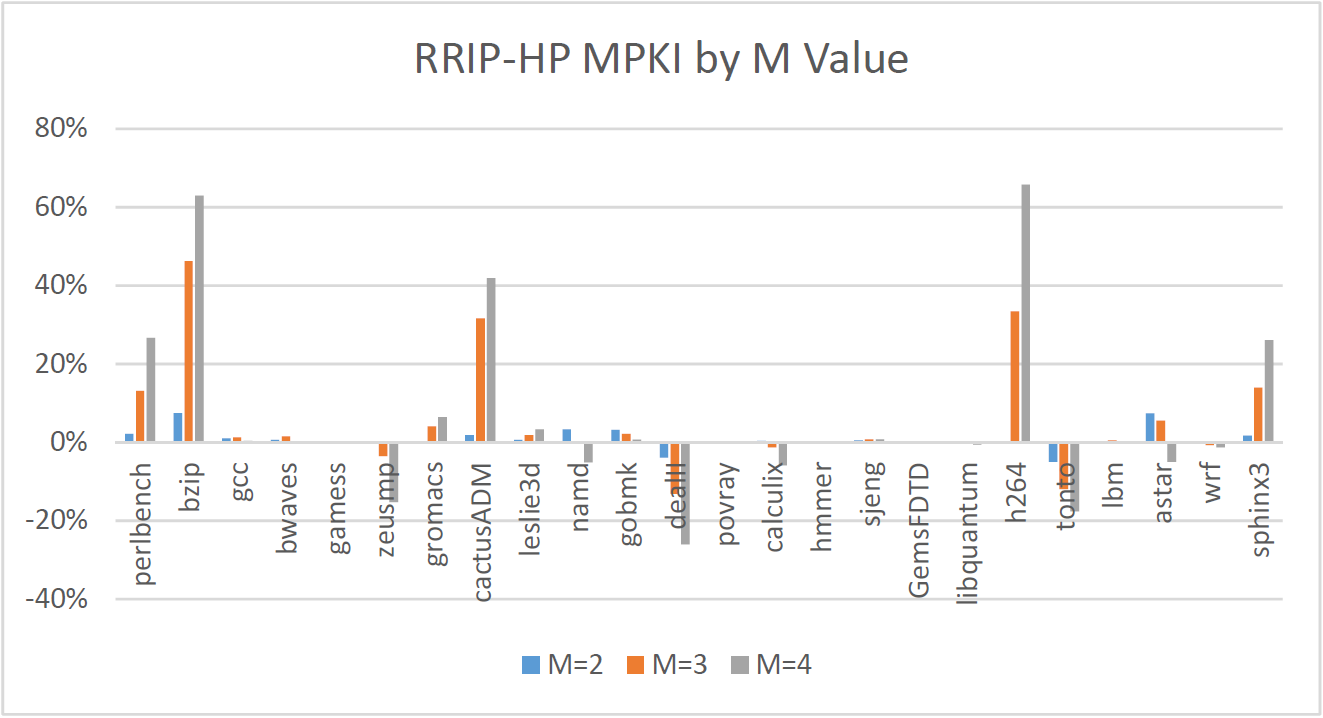
\includegraphics[width=0.49\linewidth]{rrip_hp_mpki_by_m.png}}
  \subfigure[RRIP-FP MPKI]{
    \label{rrip_fp_mpki_by_m} %% label for second subfigure
    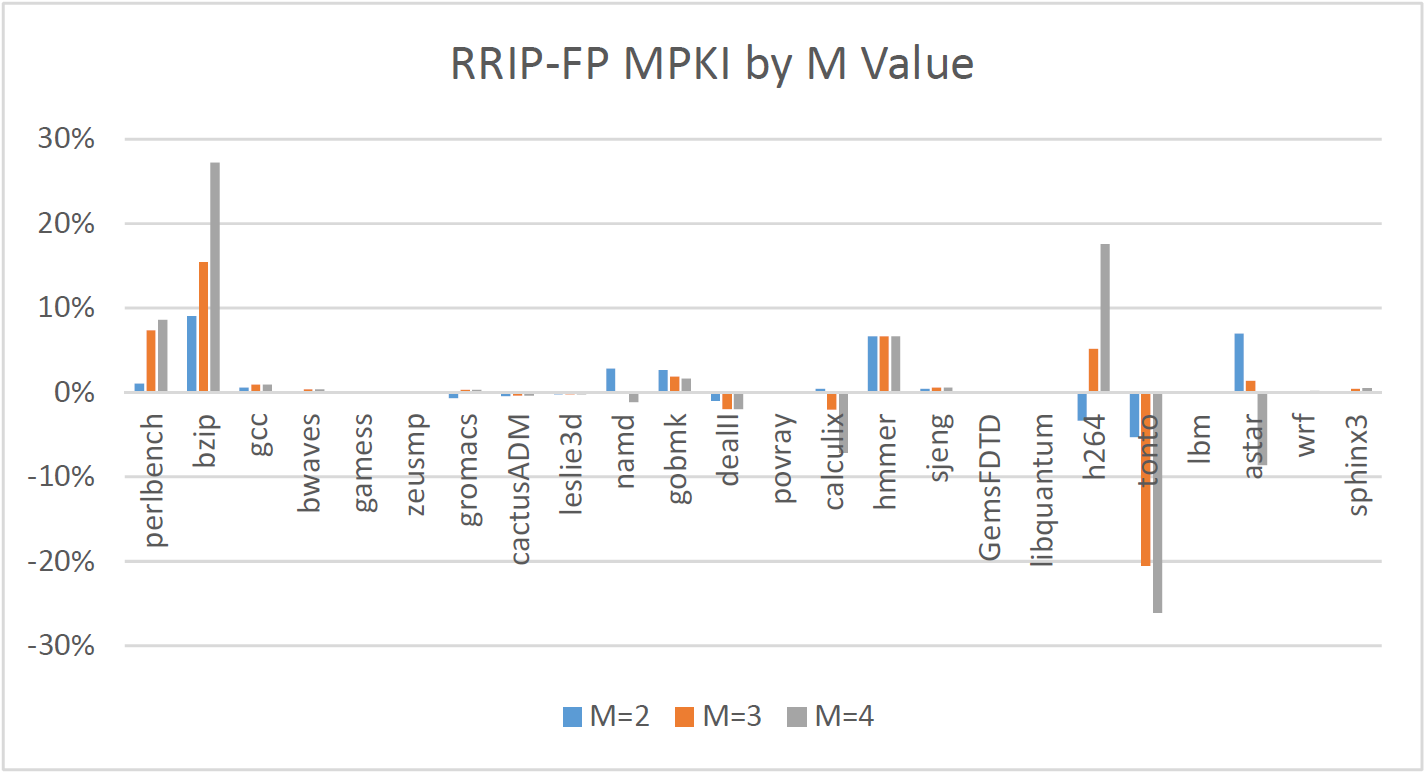
\includegraphics[width=0.49\linewidth]{rrip_fp_mpki_by_m.png}}
  \subfigure[RRIP-HP IPC]{
    \label{rrip_hp_ipc_by_m} %% label for second subfigure
    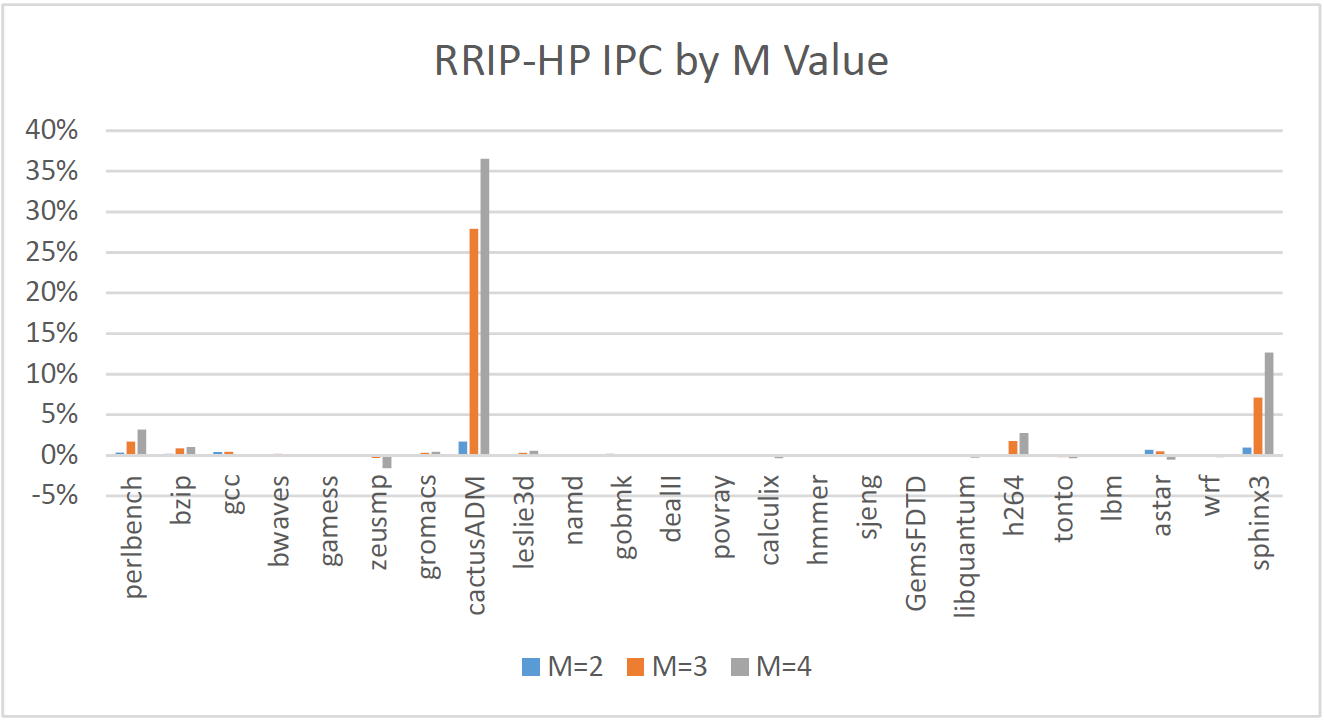
\includegraphics[width=0.49\linewidth]{rrip_hp_ipc_by_m.png}}
  \subfigure[RRIP-FP IPC]{
    \label{rrip_hp_ipc_by_m} %% label for second subfigure
    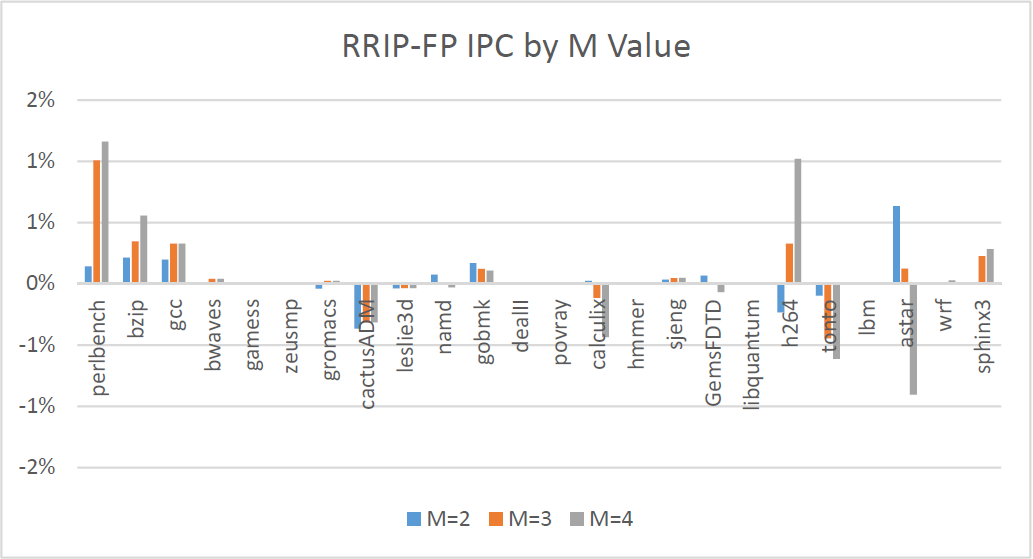
\includegraphics[width=0.49\linewidth]{rrip_fp_ipc_by_m.png}}
  \caption{RRIP performance normalized by NRU}
  \label{rrip_perf} %% label for entire figure
\end{figure*}

\subsection{Comprehensive Comparison}
Here in this section we forget all about varying $M$ value and different RRIP policies. We conducted experiments on the best policy and parameter settings currently known (i.e., RRIP-HP using $M=4$), we compared the results of such a RRIP setting with the results of NRU and we choose the normalize the performance based on LRU. The MPKI and IPC figures we got are shown in Figure \ref{rrip_nru_comp}. By doing some further statistic analysis, we can further know that: comparing to LRU, the average MPKI improvements of NRU, RRIP-HP are $1\%$ and $8\%$ respectively, the average IPC improvement of NRU is negligent but it's approximately $2\%$ when talking about RRIP-HP.
\begin{figure*}
  \centering
  \subfigure[NRU vs. RRIP-HP MPKI]{
    \label{rrip_hp_mpki_by_m} %% label for first subfigure
    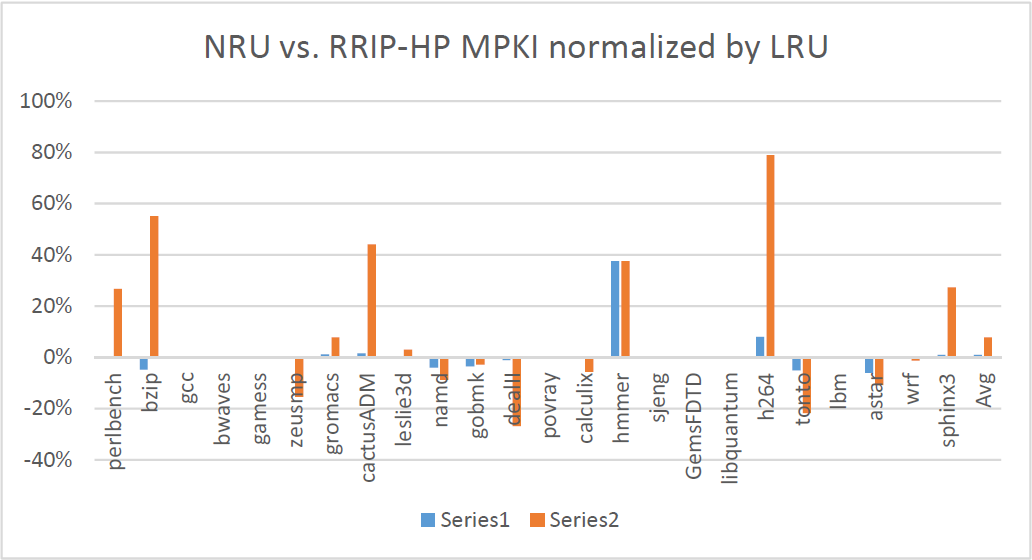
\includegraphics[width=0.49\linewidth]{nru_vs_rrip_hp_mpki.png}}
  \subfigure[NRU vs. RRIP-HP IPC]{
    \label{rrip_fp_mpki_by_m} %% label for second subfigure
    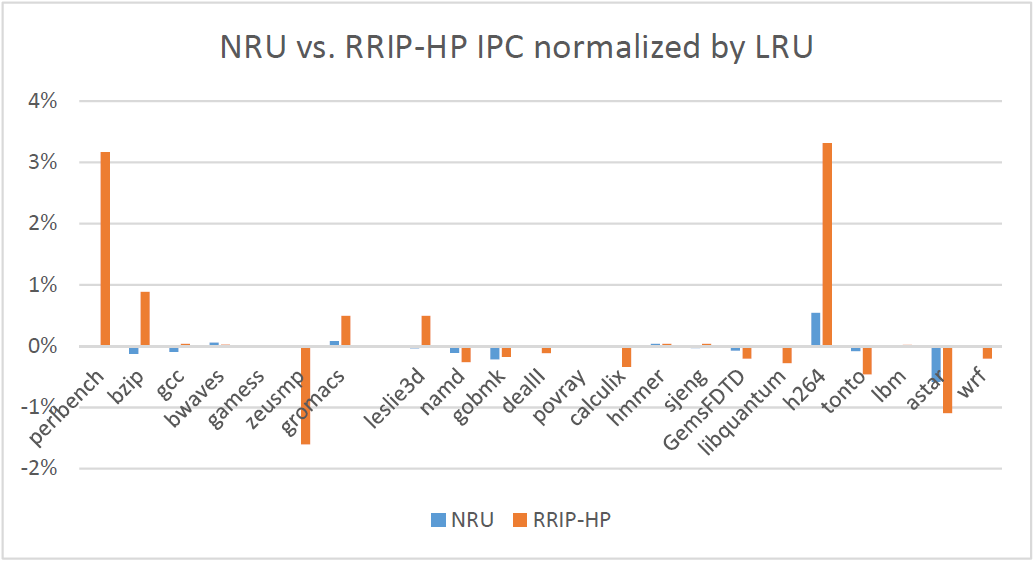
\includegraphics[width=0.49\linewidth]{nru_vs_rrip_hp_ipc.png}}
  \caption{NRU vs. RRIP-HP (M=4) normalized by NRU}
  \label{rrip_nru_comp} %% label for entire figure
\end{figure*}


% An example of a floating figure using the graphicx package.
% Note that \label must occur AFTER (or within) \caption.
% For figures, \caption should occur after the \includegraphics.
% Note that IEEEtran v1.7 and later has special internal code that
% is designed to preserve the operation of \label within \caption
% even when the captionsoff option is in effect. However, because
% of issues like this, it may be the safest practice to put all your
% \label just after \caption rather than within \caption{}.
%
% Reminder: the "draftcls" or "draftclsnofoot", not "draft", class
% option should be used if it is desired that the figures are to be
% displayed while in draft mode.
%
%\begin{figure}[!t]
%\centering
%\includegraphics[width=2.5in]{myfigure}
% where an .eps filename suffix will be assumed under latex, 
% and a .pdf suffix will be assumed for pdflatex; or what has been declared
% via \DeclareGraphicsExtensions.
%\caption{Simulation results for the network.}
%\label{fig_sim}
%\end{figure}

% Note that the IEEE typically puts floats only at the top, even when this
% results in a large percentage of a column being occupied by floats.


% An example of a double column floating figure using two subfigures.
% (The subfig.sty package must be loaded for this to work.)
% The subfigure \label commands are set within each subfloat command,
% and the \label for the overall figure must come after \caption.
% \hfil is used as a separator to get equal spacing.
% Watch out that the combined width of all the subfigures on a 
% line do not exceed the text width or a line break will occur.
%
%\begin{figure*}[!t]
%\centering
%\subfloat[Case I]{\includegraphics[width=2.5in]{box}%
%\label{fig_first_case}}
%\hfil
%\subfloat[Case II]{\includegraphics[width=2.5in]{box}%
%\label{fig_second_case}}
%\caption{Simulation results for the network.}
%\label{fig_sim}
%\end{figure*}
%
% Note that often IEEE papers with subfigures do not employ subfigure
% captions (using the optional argument to \subfloat[]), but instead will
% reference/describe all of them (a), (b), etc., within the main caption.
% Be aware that for subfig.sty to generate the (a), (b), etc., subfigure
% labels, the optional argument to \subfloat must be present. If a
% subcaption is not desired, just leave its contents blank,
% e.g., \subfloat[].


% An example of a floating table. Note that, for IEEE style tables, the
% \caption command should come BEFORE the table and, given that table
% captions serve much like titles, are usually capitalized except for words
% such as a, an, and, as, at, but, by, for, in, nor, of, on, or, the, to
% and up, which are usually not capitalized unless they are the first or
% last word of the caption. Table text will default to \footnotesize as
% the IEEE normally uses this smaller font for tables.
% The \label must come after \caption as always.
%
%\begin{table}[!t]
%% increase table row spacing, adjust to taste
%\renewcommand{\arraystretch}{1.3}
% if using array.sty, it might be a good idea to tweak the value of
% \extrarowheight as needed to properly center the text within the cells
%\caption{An Example of a Table}
%\label{table_example}
%\centering
%% Some packages, such as MDW tools, offer better commands for making tables
%% than the plain LaTeX2e tabular which is used here.
%\begin{tabular}{|c||c|}
%\hline
%One & Two\\
%\hline
%Three & Four\\
%\hline
%\end{tabular}
%\end{table}


% Note that the IEEE does not put floats in the very first column
% - or typically anywhere on the first page for that matter. Also,
% in-text middle ("here") positioning is typically not used, but it
% is allowed and encouraged for Computer Society conferences (but
% not Computer Society journals). Most IEEE journals/conferences use
% top floats exclusively. 
% Note that, LaTeX2e, unlike IEEE journals/conferences, places
% footnotes above bottom floats. This can be corrected via the
% \fnbelowfloat command of the stfloats package.




\section{Conclusion}
In practical cache replacement practice, the variety of applications cast a lot of different cache replacement challenges on our policies. Scan and thrashing are two typical examples where a portion of memory that will hardly be accessed again are referenced continuously. Under LRU policy, applications with scan and thrashing memory access patterns will degrade the cache efficiency much for it might take too many blocks that are useless in the long-term into cache, swapping blocks with a closer re-reference interval back to memory. To properly address this problem, Intel researchers proposed RRIP replacement policies which leverages historical block reference data to predict its future re-reference interval. In this paper, our work can be mainly summarized as follows:
\begin{itemize}
	\item We implemented three cache replacement policies NRU, RRIP-HP and RRIP-FP based on the descriptions in \cite{jaleel2010high}.
	\item We tested the RRIP strategies using different lengths of replacement information bits and find $M=3$ to be averagely the best bit length for both RRIP-HP and RRIP-FP.
	\item We carried out a series of benchmarks and compared performance of policies in this paper with LRU and noticed a maximum MPKI improvement about $80\%$ and a maximum IPC improvement approximately $3.5\%$.
\end{itemize}

However, there are certain cases in which the new policies suffered a worse performance than LRU or NRU, it might due to certain workload features that make it not suitable to use our new policies. Also, we didn't do much on improving those strategies since the comprehensive experiment with over 20 workloads took too much time, so we might leave those as the future work of this paper.



% conference papers do not normally have an appendix


% use section* for acknowledgment





% trigger a \newpage just before the given reference
% number - used to balance the columns on the last page
% adjust value as needed - may need to be readjusted if
% the document is modified later
%\IEEEtriggeratref{8}
% The "triggered" command can be changed if desired:
%\IEEEtriggercmd{\enlargethispage{-5in}}

% references section

% can use a bibliography generated by BibTeX as a .bbl file
% BibTeX documentation can be easily obtained at:
% http://mirror.ctan.org/biblio/bibtex/contrib/doc/
% The IEEEtran BibTeX style support page is at:
% http://www.michaelshell.org/tex/ieeetran/bibtex/
%\bibliographystyle{IEEEtran}
% argument is your BibTeX string definitions and bibliography database(s)
%\bibliography{IEEEabrv,../bib/paper}
%
% <OR> manually copy in the resultant .bbl file
% set second argument of \begin to the number of references
% (used to reserve space for the reference number labels box)
\bibliographystyle{IEEEtran}
% argument is your BibTeX string definitions and bibliography database(s)
\bibliography{refs}




% that's all folks
\end{document}


